\section{Introduzione}
Tracciare le emissioni degli algoritmi di raccomandazione e cercare di prevederle è molto importante quando si parla di sviluppo sostenibile in campo RecSys. Ancora oggi si tende a trascurare l'impatto ambientale di un'attività e, in questo ambito, si è molto propensi nell'utilizzare dei modelli molti complessi e pesanti
che richiedono molte risorse per essere addestrati ed eseguti per ottenere delle buone performance. Spesso, però, modelli molto più leggeri e semplici riescono a ottenere delle performance molto simili (se non superiori) a modelli più complessi e il tutto con un impatto ambientale decisamente minore.
Ad oggi il carbon dioxide equivalent (CO$_2$eq) è il principale indicatore utilizzato da governi e enti per misurare l'impatto ambientale di un'attività.
Il CO$_2$eq è un'unità di misura che esprime l'equivalente in CO$_2$ di tutti i gas serra emessi da un'attività, in modo da poter confrontare l'impatto ambientale di attività diverse.
Una strategia comune per calcolare il CO$_2$eq è quella di moltiplicare tra loro il \textbf{carbon intensity(CI)} e l'\textbf{energia consumata(PC)} dall'attività (nel nostro caso l'esecuzione di algoritmi).



\begin{equation*}
    \textit{emission} = \textit{CI}  \cdot \textit{PC}
\end{equation*}

\noindent In particolare i valori di CI dipendono dalle diverse fonti di energia utilizzate durante la computazione 
(es. energia solare, energia eolica, etc.). Se \textit{s} è la fonte di energia,  \textit{e$_s$} sono le emissioni per KW/h di energia e \textit{p$_s$}  è la percentuale di energia prodotta dalla fonte s, allora il CI è dato da:
\begin{equation*}
    \textit{CI} = \sum_{s \in S} \textit{e$_s$} \cdot \textit{p$_s$}
\end{equation*}

%give me author name of the paper spillo2023towards

\noindent Lo scopo di questo lavoro è quello di valutare e prevedere l'impatto ambientale di un sistema di raccomandazione (RecSys) in base alla sua sostenibilità. Per quanto riguarda la valutazione, mediante la libreria CodeCarbon\footnote{\href{http://codecarbon.io}{CodeCarbon}}{} è stato possibile misurare le emissioni prodotte dalla macchina durante l'addestramento con parametri di default per un dato modello dato un dataset. 
In questo ambito  Spillo et al.\cite{spillo2023towards} mostrano come spesso algoritmi più semplici riescono ad avere delle performance molto simili a modelli più complessi, ma con un impatto ambientale decisamente minore.
\begin{figure}[H]
    \centering
    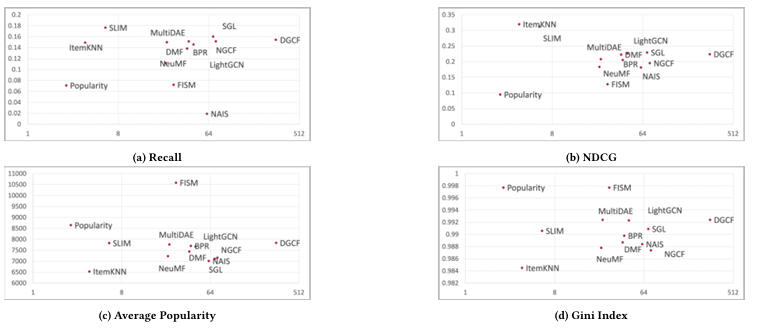
\includegraphics[scale=0.75]{images/risultati-valutazione.png}
    \caption*{Trade-off tra emissioni e performance con dataset Mind}


\end{figure}
\noindent Per quanto riguarda la previsione questo documento si propone di presentare lo stato attuale del lavoro svolto in questo ambito.
\begin{figure}[H]
    \centering
    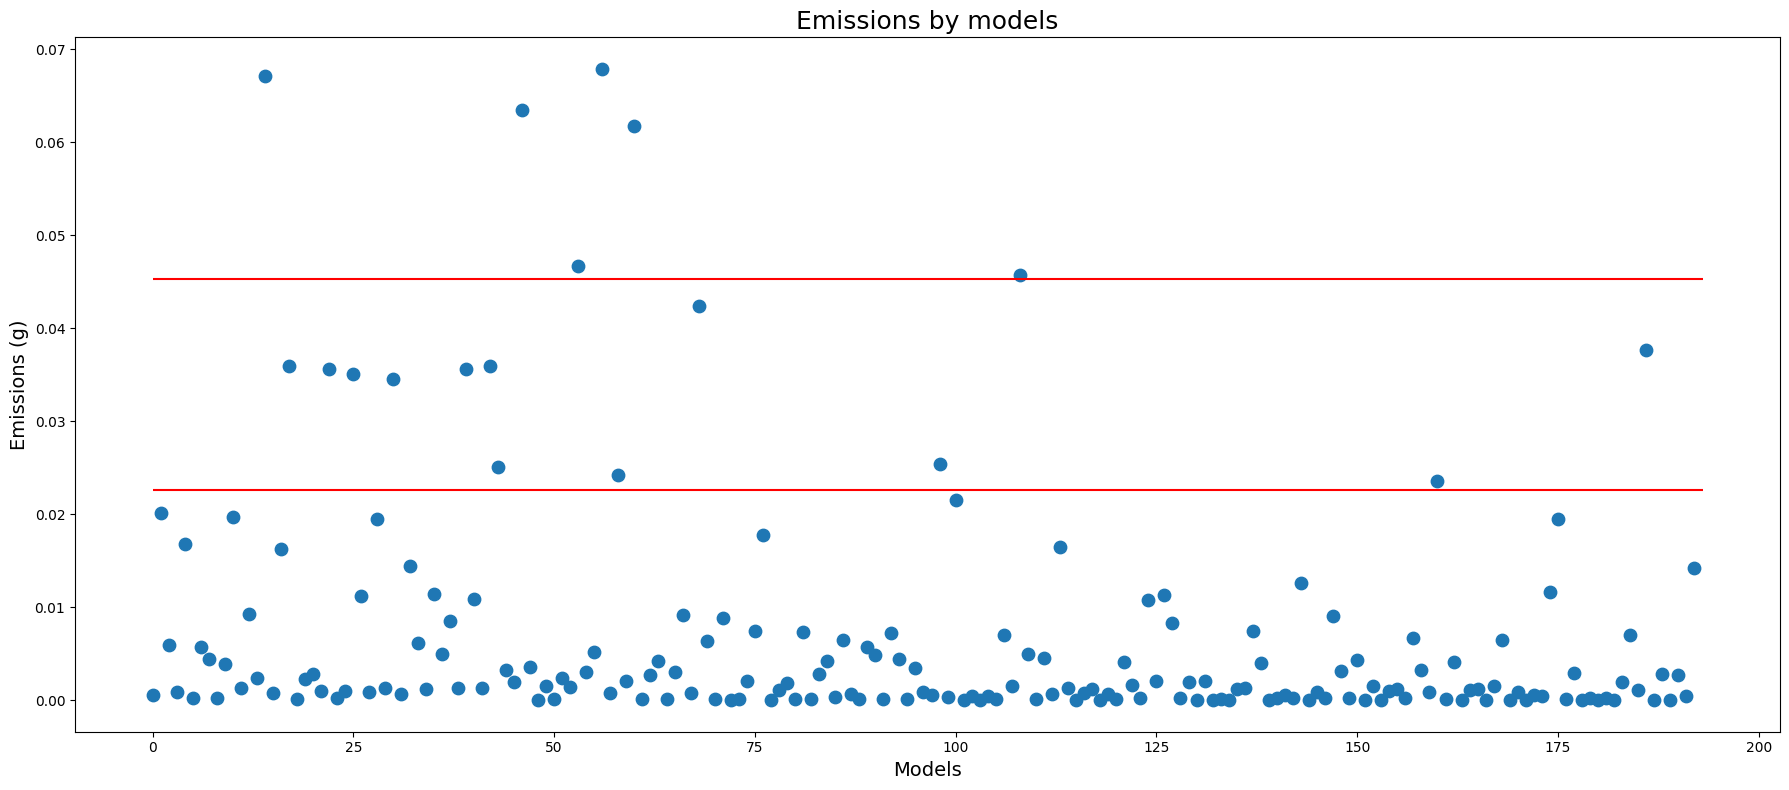
\includegraphics[scale=0.25]{images/situazione-attuale.png}
    \caption*{Emissioni prodotte dai vari modelli}
\end{figure}

\noindent L'esperimento è stato condotto su dataset presenti all'interno della libreria python RecBole\footnote{\href{http://recbole.io}{RecBole}}{}, una libreria open-source che offre un'implementazione di modelli di raccomandazione. I dataset utilizzati per l'addestramento dei modelli sono:
\begin{itemize}
    \item \textbf{MovieLens-1M}\footnote{\href{https://github.com/RUCAIBox/RecSysDatasets/blob/master/conversion_tools/usage/MovieLens.md}{Dataset MovieLens}}{}
    \item \textbf{Amazon\_Book\_60core\_kg} \footnote{\href{https://github.com/RUCAIBox/RecSysDatasets/blob/master/conversion_tools/usage/Amazon-book-KG.md}{Dataset Amazon\_Book\_60core\_kg}}{}
    \item \textbf{Mind}\footnote{\href{https://github.com/RUCAIBox/RecSysDatasets/blob/master/conversion_tools/usage/MIND.md}{Dataset MIND}}{}
\end{itemize}



